\section{Appendix: Is Multitask Deep Learning Practical for Pharma?}

\subsection{Model Training}

All deep models were trained on Stanford's Sherlock GPU cluster via DeepChem. Models were trained for at most a day on a single GPU per model,
following guidelines that longer training times would render model training too unwieldy to use in practice at pharmaceutical companies \cite{ma2015deep}.  Rectified linear unit activations are used for all models.


\subsection{Kaggle Architectures}
Multitask architectures for the Kaggle collection had three hidden layers of sizes $2000, 1000, 1000$. All hidden layers had dropout of $.25$. Weights were initialized with normal distributions of mean zero and standard deviation $.02$, truncated two standard deviations away from mean. Biases were initialized as $1$. $L^2$ weight decay of size $.0004$ was applied during training. Models were trained with learning rate $3e-5$ for 100 epochs with ADAM. Singletask models had the same architecture.

Bypass models had three shared hidden layers of size $2000, 1000, 1000$, and had three per-task bypass layers of size $200$. All other parameters were identical to multitask architectures.

Progressive models had $100$ hidden units per task, and were trained with learning rate $3e-4$, and $L^2$ penalty of $.0001$. All other parameters were identical to multitask architecture.

\subsection{Factors Architectures}
Multitask architectures for the Factors collection had three hidden layers of sizes $1000, 1000, 1000$. All hidden layers had dropout of $.25$. Weights were initialized with normal distributions of mean zero and standard deviation $.02$, truncated two standard deviations away from mean. Biases were initialized as $1$. $L^2$ weight decay of size $.0001$ was applied during training. Models were trained with learning rate $3e-4$ for 125 epochs with ADAM. Singletask models had the same architecture and were also trained for 125 epochs.

Bypass models had three shared hidden layers of size $1000, 1000, 1000$, and had three per-task bypass layers of size $100$. All other parameters were identical to multitask architectures.

Progressive models had $750$ hidden units per task, and were trained with learning rate $3e-4$, and $L^2$ penalty of $.0001$. All other parameters were identical to multitask architecture.

\subsection{Kinase Architectures}
Multitask architectures for the Kinase collection had three hidden layers of sizes $1000, 1000, 1000$. All hidden layers had dropout of $.25$. Weights were initialized with normal distributions of mean zero and standard deviation $.02$, truncated two standard deviations away from mean. Biases were initialized as $.5$. $L^2$ weight decay of size $.0001$ was applied during training. Models were trained with learning rate $3e-4$ for 50 epochs with ADAM. Singletask models had the same architecture.

Bypass models had three shared hidden layers of size $500, 500, 500$, and had three per-task bypass layers of size $20$. All other parameters were identical to multitask architectures.

Progressive models had $50$ hidden units per task, and were trained with learning rate $3e-4$, and $L^2$ penalty of $.0001$. All other parameters were identical to multitask architecture.

\subsection{UV Architectures}
Multitask architectures for the UV collection had three hidden layers of sizes $1000, 1000, 1000$. All hidden layers had dropout of $.25$. Weights were initialized with normal distributions of mean zero and standard deviation $.02$, truncated two standard deviations away from mean. Biases were initialized as $1.$. $L^2$ weight decay of size $.0001$ was applied during training. Models were trained with learning rate $3e-4$ for 50 epochs with ADAM. Singletask models had the same architecture, but were trained for $30$ epochs.

Bypass models had three shared hidden layers of size $500, 500, 500$, and had three per-task bypass layers of size $20$. All other parameters were identical to multitask architectures.

\newpage
\subsection{For Table of Contents Use Only}
{\huge Is Multitask Deep Learning Practical for Pharma?}

{\Large Bharath Ramsundar, Bowen Liu, Zhenqin Wu, Andreas Verras, Matthew Tudor, Robert P. Sheridan, Vijay Pande}

\begin{figure}[H]
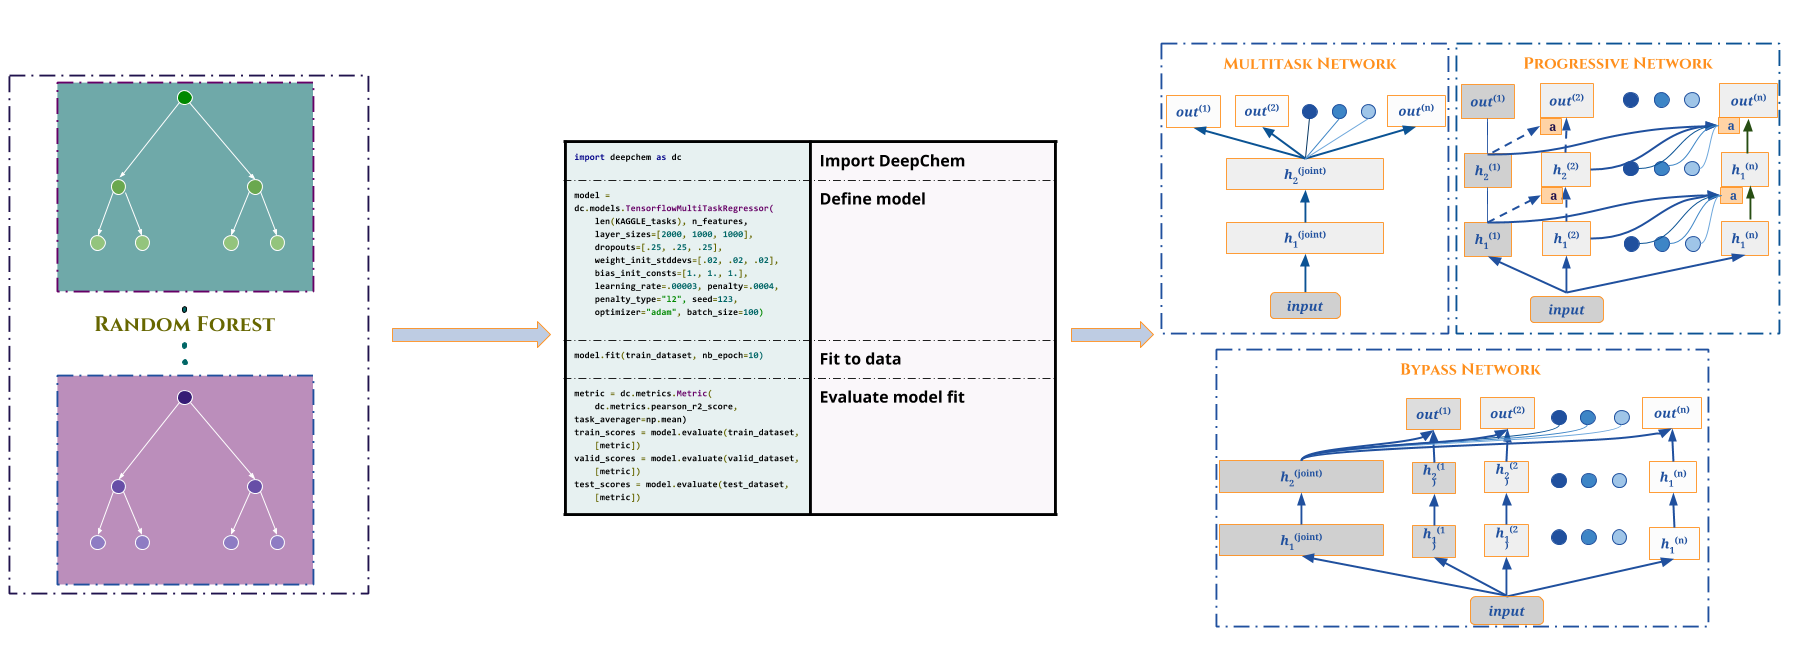
\includegraphics[scale=0.25]{Images/multitask_TOC.png}
\end{figure}

Synopsis: Multitask deep learning has emerged as a powerful tool for computational drug discovery. However, despite a number of preliminary studies, multitask deep networks have yet to be widely deployed in the pharmaceutical and biotech industries. Our work aims to facilitate adoption by introducing a high-quality open-source implementation of multitask deep networks as part of the DeepChem open-source platform. Our implementation enables simple python scripts to construct, fit, and evaluate sophisticated deep models.
